\chapter*{Introduction}
Although the title of this work is very general; the principal objective of this project is to determine the orbit followed by a particle around a slowly rotating weak gravitational source. By being specific, with ``weak gravitational source'' we mean that the central body generates a weak gravitational field, therefore is not necessary to work with the general Einstein equations and the Post-Newtonian (PN) approximation is enough to determine the motion of the particle. We work up to the 1PN order. \cite{ GravityPoisson, Weinberg, Theoryandexperiments}\\

In Chapter \ref{ch: celestial mechanics} we introduce the two-body problem, the perturbation theory, and the respective orbital elements for Classical Celestial Mechanics. The most relevant conclusion of this chapter is to introduce the general position in space of the orbit, determined by both the $x$, $y$, and $z$ positions, and the time-dependent basis; finally, we give the derivative with respect to the true anomaly of the orbital elements. Continuing with the Linearized theory in Chapter \ref{ch: firstchapter} in which we introduce the principal characteristics of a gravitational source that can be considered as a weak field and some relevant aspects of the Energy-Momentum Tensor of a system modeled as a perfect fluid. Since we are working with a weak field, the metric is introduced as a perturbation to the Minkowski metric, and the small parameter that gives the order of expansion of the metric is also introduce. We write the Einstein Field Equations under this approximation and determine the potentials involved in these, in terms of the Energy-Momentum Tensor. The metric is expanded in terms of the potentials, and these are written in terms of the expanded Energy Momentum Tensor; all the expression are written considering the Standard Post-Newtonian gauge.\cite{GravityPoisson} \\

The problem of one body following, the Schwarzschild metric, is developed in Chapter \ref{ch:chapter2}. We introduce the general form of the Lagrangian, the equations of motion under 1PN approximation and the concept of parametrize metric. The respective perturbing force and orbital elements are calculated.\\

The previous chapters have the purpose of introducing and provide enough resources to develop the main objective of the work. In Chapter \ref{ch: rotation} er introduce some relevant aspects of the Kerr Metric \cite{Bambi, Frolov, Raine} and the Weyl Levi Civita Metric \cite{johnandcoulter}, with the latter determines the Newtonian potential for a non-spherically symmetric and axially symmetric body until quadrupole moment. Then we deduce the same potential but following the classical approach to determine the form of the quadrupole moment in terms of the inertia moments \cite{Goldstain, GravityPoisson}. The potentials needed to write the Post-Newtonian metric of this system are calculated considering a slowly rotating body; therefore, we only consider the first order of quadrupole moment and rotational velocity. The metric is parametrized following the one showed in \cite{Brumberg}. We construct the perturbing force and its respective projections on the time dependent basis. The force is divided into four different types of contributions: the one corresponding to the Newtonian quadrupole, the Schwarzschild perturbation, the one due to the rotation of the central body, and the relativistic quadrupole perturbation \cite{Brumberg}. The final part of this chapter consists in calculate the secular changes of the orbital elements. The secular changes corresponding to the Newtonian quadrupole correspond to the ones showed in the literature.\\

The project is concluded by showing, in the last Chapter, how  the secular changes determine in the previous chapter, are applied to the system Earth + Satellite in two of the most famous types of orbit, the Geostationary and the Molniya. We plot the changes in terms of the orbital period and the 3D orbit for different angles of view.\\

Some of the algebraic steps were made using Mathematica, the plots in Chapter \ref{ch: applications} were made using Python via a Jupyter Notebook. These computational resources, as well as the \LaTeX  \hspace{0.2cm} documents, can be found in \url{https://github.com/taceroc/PPN-Slowly-rotation.git}.




\chapter{Celestial Mechanics}\label{ch: celestial mechanics}

\section{Two Body Problem}

A two body system, as in Figure \ref{fig: twobodysystem}, can be described following the Newtonian formalism. This system is characterized by the newtonian potential,
\begin{align}
	\phi (r) = -\frac{GM}{r},
\end{align}
where $M$ is the total mass of the system.
\begin{figure}[htb!]
\centering
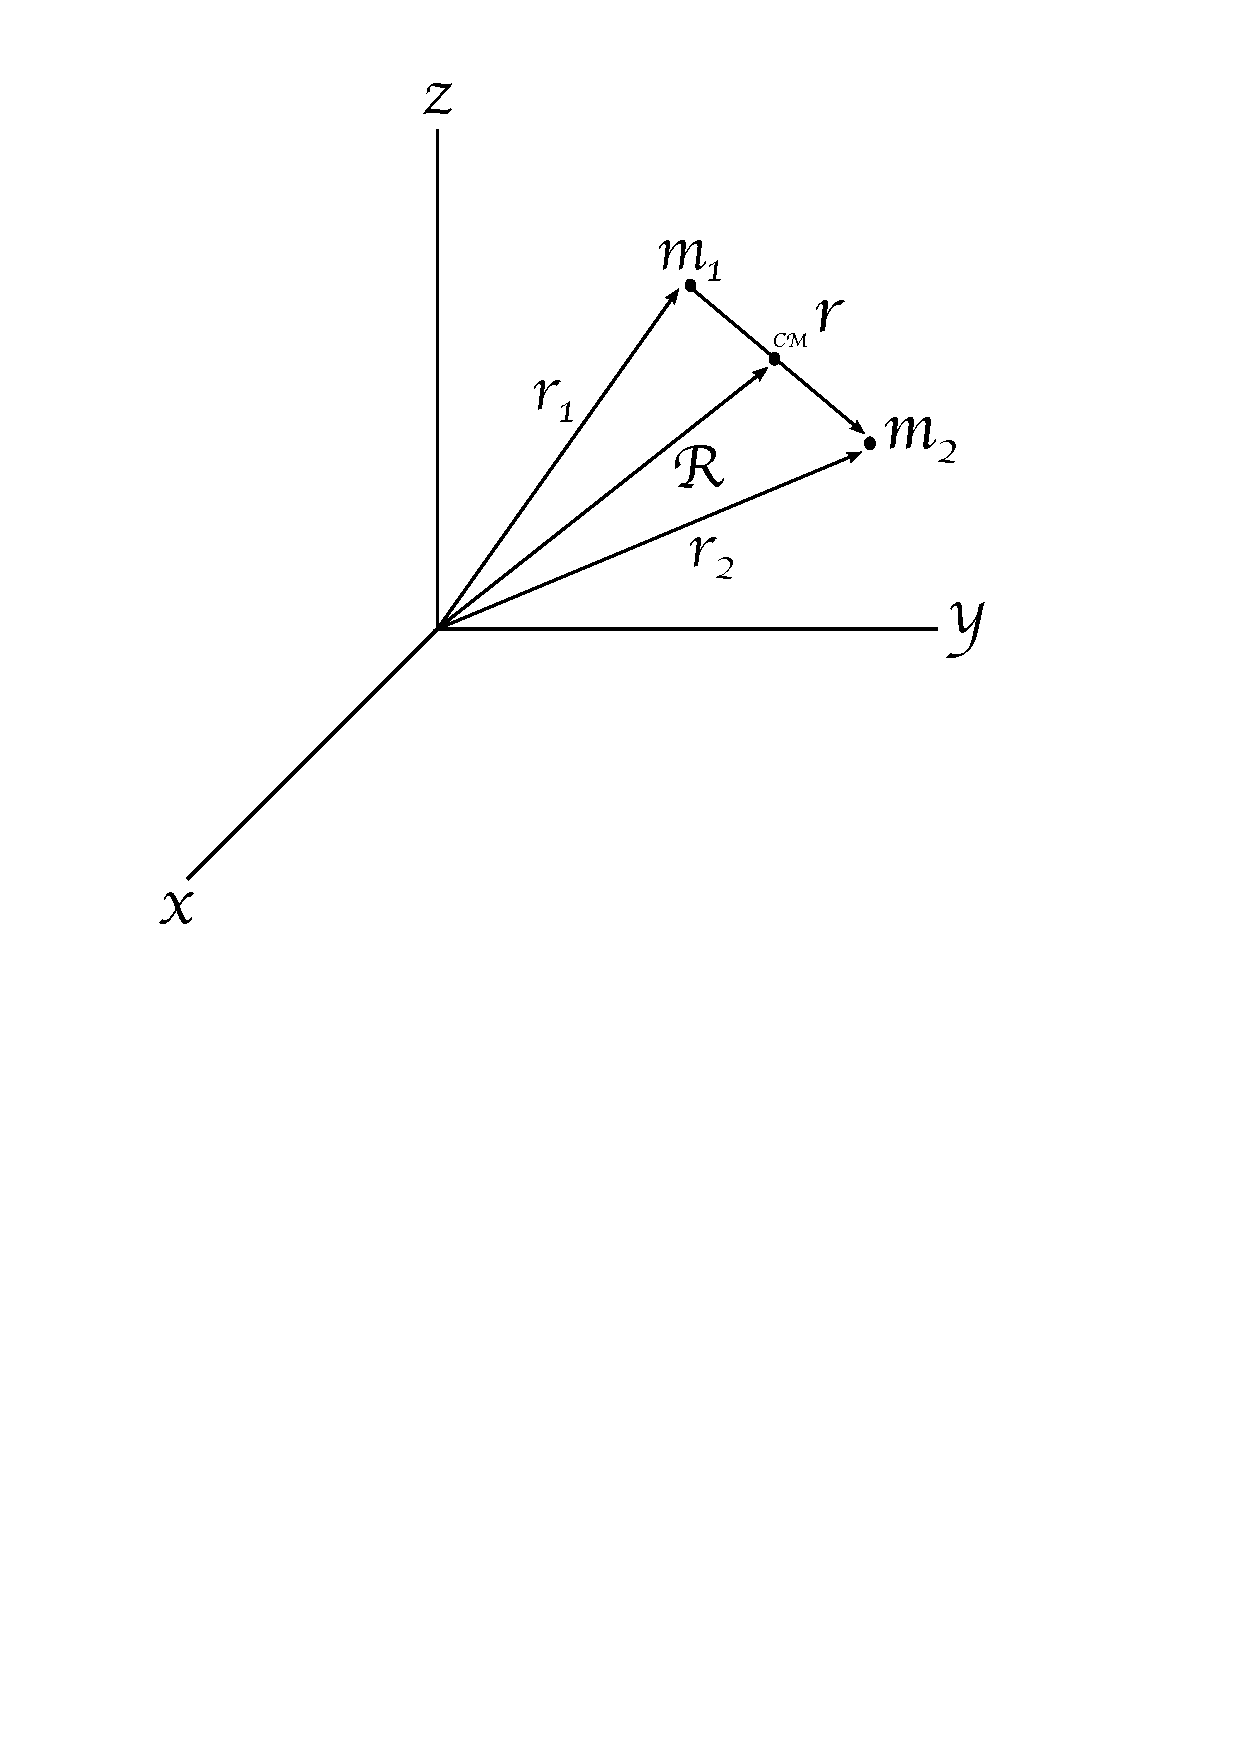
\includegraphics[width=7cm]{../Tesis/Capitulo0/Figures/Coordenadas.pdf}
\caption{Two body system}
\label{fig: twobodysystem}
\end{figure}

The equation of motion is as usual
\begin{align}
	\ddot{\mathbf{x}} = -\frac{GM}{r^3} \mathbf{x}.
	\label{eq: newtonianeqmotion}
\end{align}

Note here that $\mathbf{x} = (x,y,z)$, and the equation of motion is of second order; therefore, to determine in a univocal form the orbit of the system, it is necessary to find six constants of motion.\\

Following the Euler-Lagrange formalism it is found that the angular momentum is a conserved quantity. The plane of motion; defined by the radial direction and the velocity, and according to the definition of angular momentum $\mathbf{L} = \mathbf{x} \times \dot{\mathbf{x}}$; is constant over time, then the motion of the system is fixed in a plane, and the angular momentum is perpendicular to that plane as shown in Figure \ref{fig: tplanfijo}.\\

\begin{figure}[htb!]
\centering
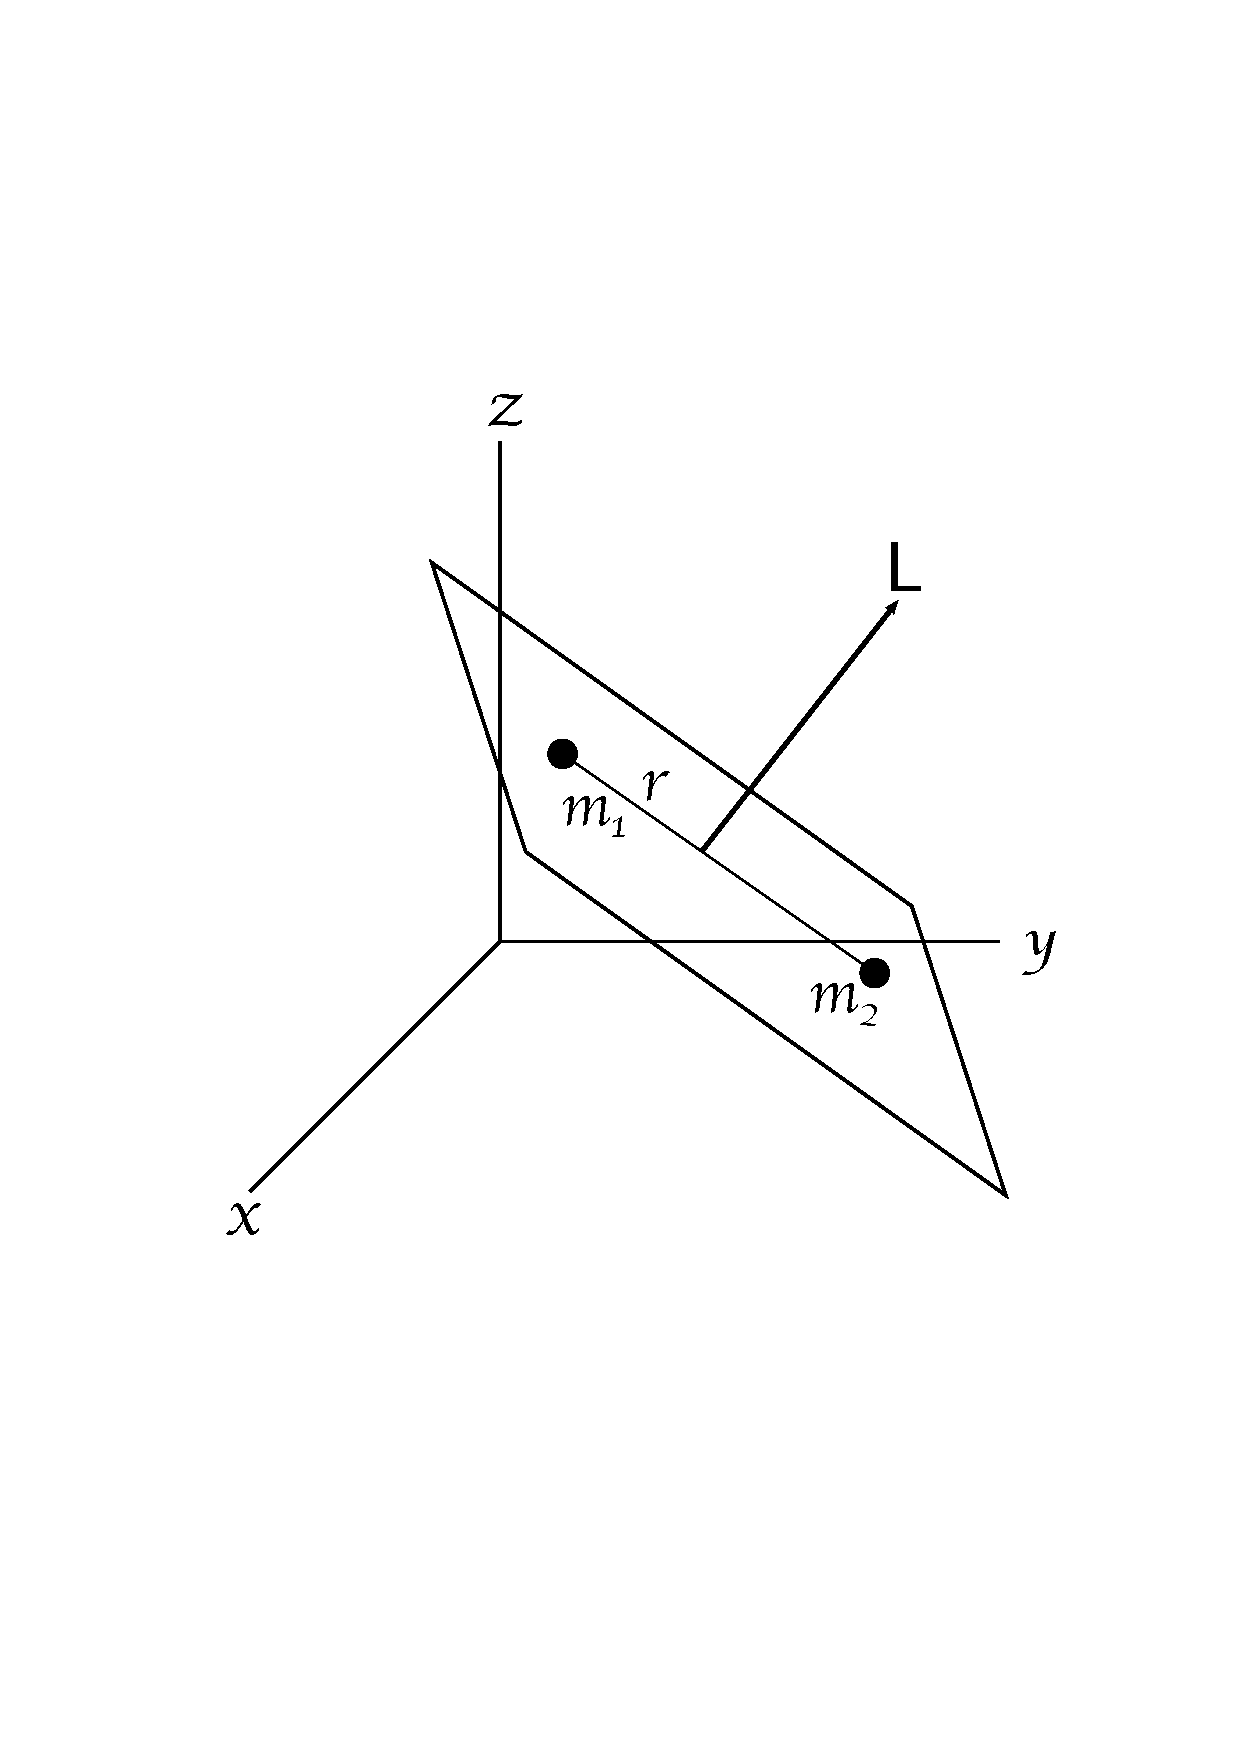
\includegraphics[width=7cm]{../Tesis/Capitulo0/Figures/Planofijo.pdf}
\caption{Plane of motion of the two body system}
\label{fig: tplanfijo}
\end{figure}

From the fact mentioned above, it is possible to introduce a new coordinate system in which the system lies on a $\mathcal{X}\mathcal{Y}$ plane and the angular momentum is on the $\mathcal{Z}$ direction, perpendicular to that plane. The motion is now described by the polar coordinates $r$ and $\phi$, where $\mathbf{r} = (r \cos\phi, r \sin\phi, 0)$. It is useful and more practical to describe the motion with a time dependent basis,
\begin{subequations}
\label{eq: timedependentbasisnopertur}
\begin{align}
&\mathbf{n} = (\cos\phi, \sin\phi,0)  = \frac{\mathbf{r}}{r}\\
&\boldsymbol{\lambda} = (-\sin\phi, \cos\phi,0), \hspace{1cm} \frac{d\mathbf{n}}{d\phi} = \boldsymbol{\lambda}\\
&\mathbf{k} = (0,0,1).
\end{align}
\end{subequations}


The equation of the trajectory for the two body system is
\begin{align}
u '' + u =\frac{GM}{\ell ^{\,2}}, \hspace{1cm} u(\phi) = \frac{1}{ r (\phi)},
\end{align}
where $\ell$ is the total angular momentum per unit mass.\\

The solution of this equation is the well know conic sections,
\begin{align}
r (\phi) = \frac{p}{1+e\cos(\phi+\omega)}
\end{align}
where $e$ and $\omega$ are integration constants. Particularly, for elliptic orbits we have that \begin{align}
p = a(1-e^2) = \frac{\ell^2}{GM},
\end{align}
where $a$ is a constant of integration, corresponding to the semi-major axis.

\section{Orbital elements}
A a general description of the motion of the system can be done by considering a coordinates $(x,y,z)$, where the orbit is not longer defined in the $\mathcal{X}\mathcal{Y}$ plane. The orbit is completely defined by knowing the six orbital elements:
\begin{enumerate}\bfseries
\color{forestgreen}
\item  a: semi-major axis,
\item e: eccentricity,
\item $\boldsymbol{\omega}$: argument of the pericenter,
\item $\boldsymbol{\iota}$: inclination,
\item $\boldsymbol{\Omega}$: longitude of the ascending node,
\item T: orbital period (in general a time constant).
\end{enumerate}

\begin{figure}[htb!]
\centering
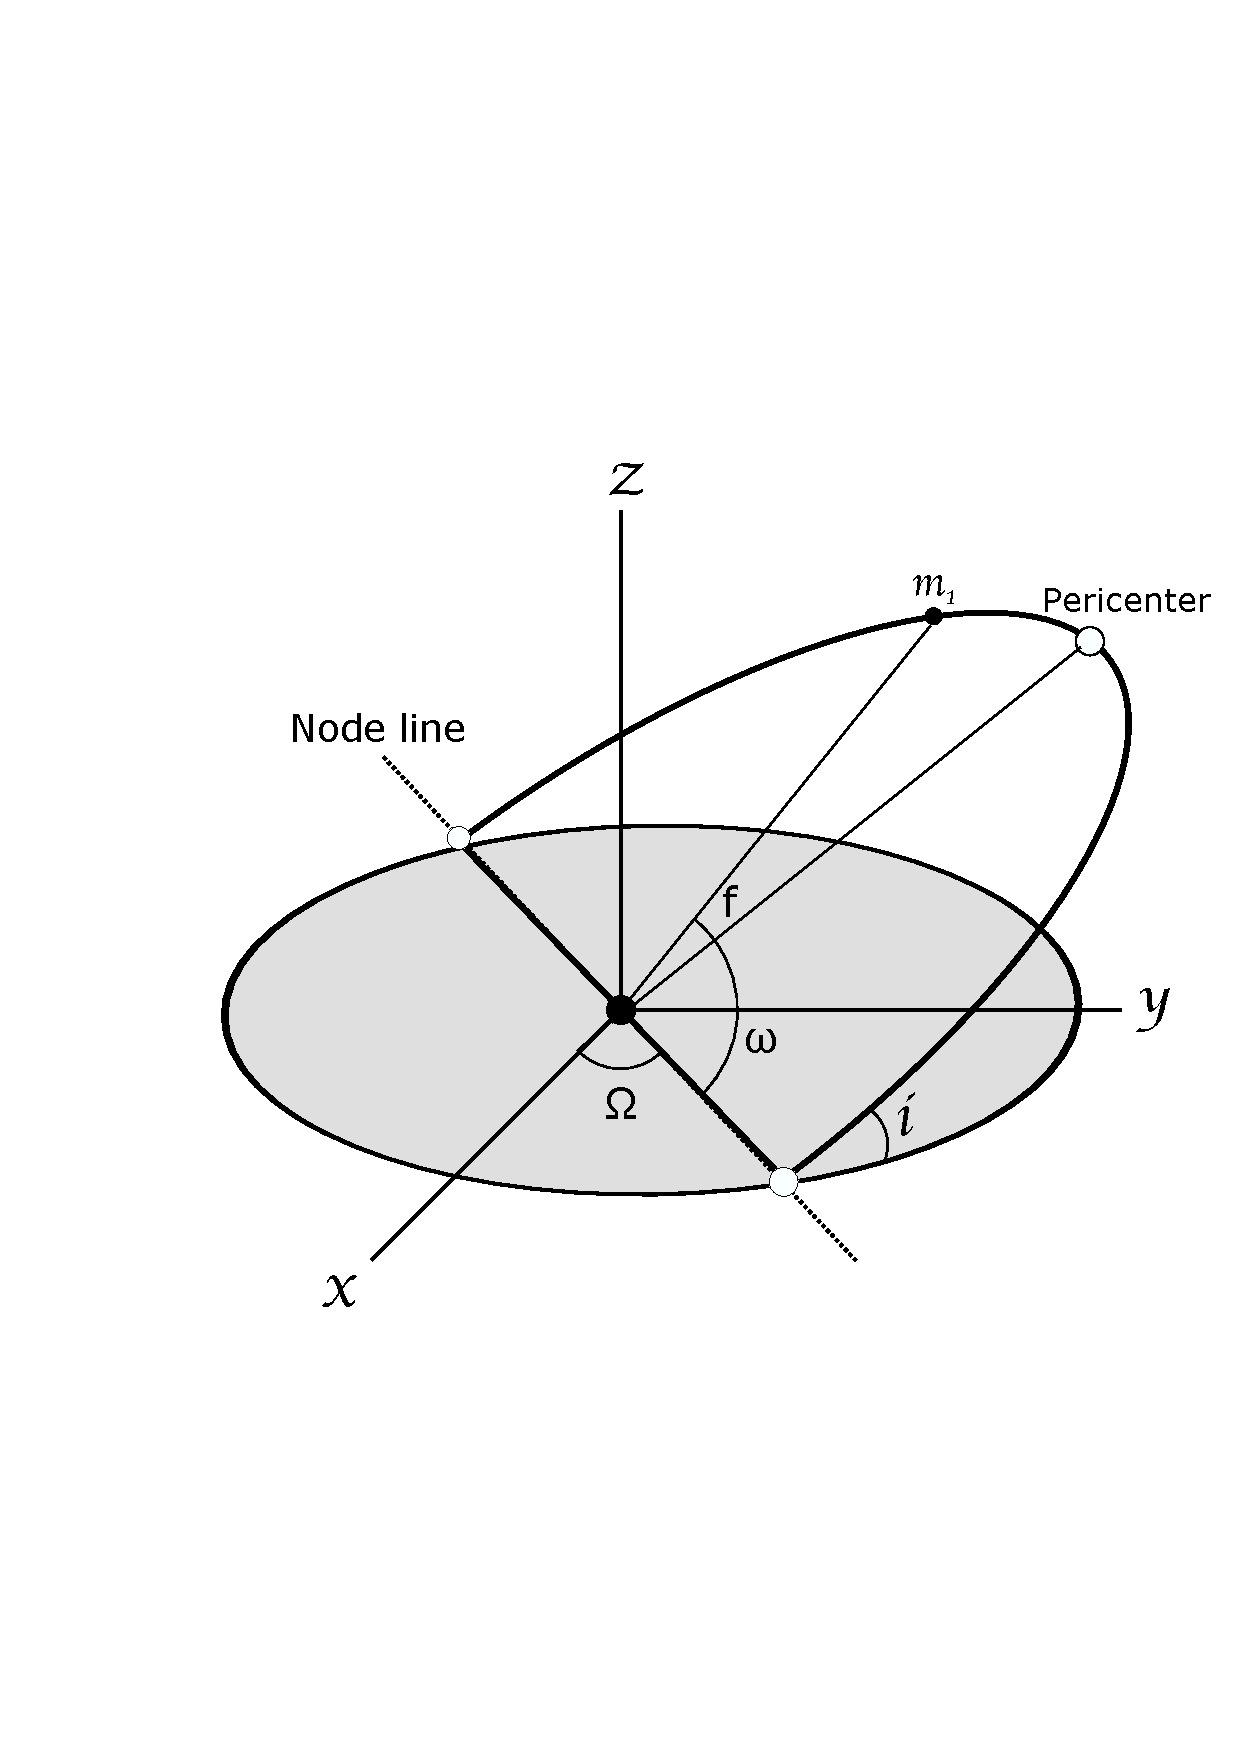
\includegraphics[width=7cm]{../Tesis/Capitulo2/Figures/elementosorbitales.pdf}
\caption{Configuration of the general coordinate system}
\label{fig: orbitalelementsdibujo}
\end{figure}

The semi-major axis and eccentricity described the geometry of the orbit. For elliptical orbits, the eccentricity has values between $0$ and $1$. $\omega$, $\iota$ and $\Omega$ describe the position of the orbit in the general system and a constant related to time.\\

The procedure to determine the connection between the $\mathcal{X}\mathcal{Y}$ and the general coordinates $xyz$ is applying the following rotations:

\begin{align}
\begin{bmatrix}
x\\
y\\
z\end{bmatrix}
= 
\begin{bmatrix}
\cos \Omega & -\sin \Omega & 0 \\
\sin \Omega & \cos\Omega & 0\\
0&0&1
\end{bmatrix}
\begin{bmatrix}
1&0&0\\
0&\cos \iota & -\sin \iota \\
0& \sin \iota & \cos\iota 
\end{bmatrix}
\begin{bmatrix}
\cos \omega & -\sin {\omega} & 0 \\
\sin \omega & \cos\omega & 0\\
0&0&1
\end{bmatrix}
\begin{bmatrix}
\mathcal{X}\\
\mathcal{Y}.\\
0\end{bmatrix}
\end{align}

The time dependent basis, in the general coordinate system, as shown in Figure \ref{fig: tplanfijo} are:\\

In the radial direction, $\mathbf{n}$, where the angle $\phi$ in equations (\ref{eq: timedependentbasisnopertur}) is replace by the letter $f$, and is known as true anomaly,
\begin{align*}
\begin{bmatrix}
n_x\\
n_y\\
n_z\end{bmatrix}
= 
\begin{bmatrix}
\cos \Omega & -\sin \Omega & 0 \\
\sin \Omega & \cos\Omega & 0\\
0&0&1
\end{bmatrix}
\begin{bmatrix}
1&0&0\\
0&\cos \iota & -\sin \iota \\
0& \sin \iota & \cos\iota 
\end{bmatrix}
\begin{bmatrix}
\cos \omega & -\sin {\omega} & 0 \\
\sin \omega & \cos\omega & 0\\
0&0&1
\end{bmatrix}
\begin{bmatrix}
\cos f\\
\sin f\\
0\end{bmatrix},
\end{align*}

\begin{align}
\begin{split}
	\mathbf{n} =& [\cos \Omega \cos (f +\omega) - \cos \iota \sin \Omega \sin (f+\omega)] \mathbf{\hat{e}_x}\\
	+& [\sin \Omega \cos (f +\omega) + \cos \iota \cos \Omega \sin (f+\omega)] \mathbf{\hat{e}_y}\\
	+ & [ \sin \iota  \sin (f+\omega)] \mathbf{\hat{e}_z}.
	\end{split}
\label{eq: nunitary}
\end{align}

The $\boldsymbol{\lambda}$ direction,
\begin{align*}
\begin{bmatrix}
\lambda_x\\
\lambda_y\\
\lambda_z\end{bmatrix}
= 
\begin{bmatrix}
\cos \Omega & -\sin \Omega & 0 \\
\sin \Omega & \cos\Omega & 0\\
0&0&1
\end{bmatrix}
\begin{bmatrix}
1&0&0\\
0&\cos \iota & -\sin \iota \\
0& \sin \iota & \cos\iota 
\end{bmatrix}
\begin{bmatrix}
\cos \omega & -\sin {\omega} & 0 \\
\sin \omega & \cos\omega & 0\\
0&0&1
\end{bmatrix}
\begin{bmatrix}
-\sin f\\
\cos f \\
0\end{bmatrix},
\end{align*}


\begin{align}
\begin{split}
	\boldsymbol{\lambda} =& [-\cos \Omega \sin (f +\omega) - \cos \iota \sin \Omega \cos (f+\omega)] \mathbf{\hat{e}_x}\\
	+& [-\sin \Omega \sin (f +\omega) + \cos \iota \cos \Omega \cos (f+\omega)] \mathbf{\hat{e}_y}\\
	+ & [ \sin \iota  \cos (f+\omega)] \mathbf{\hat{e}_z}.
	\end{split}
\label{eq: lambdaunitary}
\end{align}

The $\mathbf{k}$ direction,
\begin{align*}
\begin{bmatrix}
k_x\\
k_y\\
k_z\end{bmatrix}
= 
\begin{bmatrix}
\cos \Omega & -\sin \Omega & 0 \\
\sin \Omega & \cos\Omega & 0\\
0&0&1
\end{bmatrix}
\begin{bmatrix}
1&0&0\\
0&\cos \iota & -\sin \iota \\
0& \sin \iota & \cos\iota 
\end{bmatrix}
\begin{bmatrix}
\cos \omega & -\sin {\omega} & 0 \\
\sin \omega & \cos\omega & 0\\
0&0&1
\end{bmatrix}
\begin{bmatrix}
0\\
0 \\
1\end{bmatrix},
\end{align*}

\begin{align}
	\mathbf{k} =& \sin \iota \sin \Omega  \mathbf{\hat{e}_x}
	 -\sin \iota \cos \Omega \mathbf{\hat{e}_y}
	 + \cos \iota \mathbf{\hat{e}_z}.
\label{eq: kunitary}
\end{align}


The position is given by,
\begin{align}
\begin{split}
	\mathbf{x} =& r [\cos \Omega \cos (f +\omega) - \cos \iota \sin \Omega \sin (f+\omega)] \mathbf{\hat{e}_x}\\
	+&r [\sin \Omega \cos (f +\omega) + \cos \iota \cos \Omega \sin (f+\omega)] \mathbf{\hat{e}_y}\\
	+ & r[ \sin \iota  \sin (f+\omega)] \mathbf{\hat{e}_z},
	\end{split}
\label{eq: xgeneral}
\end{align}

and its derivative with respect to time is

\begin{align}
\begin{split}
	\dot{\mathbf{x}} =&-\sqrt{ \frac{GM}{p}} [\cos \Omega (\sin  (f +\omega) + e \sin \omega) + \cos \iota \sin \Omega  (\cos  (f +\omega) + e \cos \omega)] \mathbf{\hat{e}_x}\\
	-&\sqrt{ \frac{GM}{p}} [\sin \Omega (\sin  (f +\omega) + e \sin \omega) - \cos \iota \cos \Omega  (\cos  (f +\omega) + e \cos \omega)] \mathbf{\hat{e}_y}\\
	- & \sqrt{ \frac{GM}{p}} \sin \iota [  \cos (f+\omega) + e\cos \omega] \mathbf{\hat{e}_z}.
	\end{split}
\label{eq: dotxgeneral}
\end{align}

The gray plane in Figure \ref{fig: orbitalelementsdibujo}, known as Reference plane, can be the Ecliptic plane (Sun at center), Equatorial plane (Earth at center) or Galactic plane. The $x$ axis usually refers to the $\Upsilon$: First point of Aries, which is the point, seen by an observer on the Earth, where the Sun crosses the equator from south to north. \cite{Clarke}\\

The orbital elements can be found with the quantities and vectors above as follows,
\begin{align}
a &= \frac{p}{1-e^2} \\
\cos \iota &= \mathbf{k} \cdot \mathbf{\hat{e}_z}\\
\sin \iota \sin \Omega &=  \mathbf{k} \cdot \mathbf{\hat{e}_x}\\
\sin \iota \sin \omega &=  \frac{\mathbf{e} \cdot \mathbf{\hat{e}_z}}{e}.
\end{align}
The eccentricity can be found via the Laplace - Runge -Lenz vector, defined as
\begin{align}
\mathbf{e} = \frac{\dot{\mathbf{x}}  \times \boldsymbol{\ell}}{GM} - \mathbf{n}.
\end{align}

\section{Perturbation Theory}

 For the two body system, the orbital elements are constant over time. Introducing a perturbation to the system, such a third body, relativistic, quadrupole effects, etc., the elements are now dependent of time. A perturbing force, smaller than the newtonian force, must be added to the force given by the two body system in (\ref{eq: newtonianeqmotion}) [\cite{Brumberg, Sergeiclassical}],
\begin{align}
	\ddot{\mathbf{x}} = -\frac{GM}{r^2} \mathbf{n} + \mathbf{F}.
\end{align}
 
The force can be decomposed in terms of the time dependent basis as
\begin{align}
	\mathbf{F} = \mathcal{R} \mathbf{n} + \mathcal{T} \boldsymbol{\lambda}+ \mathcal{W}\mathbf{k}.
\end{align}

The first order correction to the orbital elements in terms of, the true anomaly are \cite{Brumberg, Larranaga}

\begin{subequations}\label{eq:OsculatingOrbitalElementsinf}
\begin{align}
\frac{da}{df} &= \frac{2(1-e^2)}{n^2} \left[ \frac{e \sin f }{(1+e \cos f)^2}\mathcal{R} + \frac{1}{1+e\cos f} \mathcal{T} \right] \\
\frac{de}{df} &= \frac{(1-e^2)^2}{n^2a} \left[ \frac{\sin f}{(1+e \cos f)^2} \mathcal{R} + \frac{2\cos f + e \left( 1 + \cos^2 f \right) }{(1 + e\cos f)^3} \mathcal{T} \right] \\
\frac{d \iota}{df} &= \frac{(1-e^2)^2}{n^2 a} \frac{\cos (f+\omega)}{(1+e\cos f)^3} \mathcal{W} \\
\frac{d \Omega}{df} &= \frac{(1-e^2)^2}{n^2 a}  \frac{\sin (f+\omega)}{(1+e\cos f)^3 \sin \iota } \mathcal{W} \\
\frac{d\omega}{df} &=\frac{(1-e^2)^2}{n^2 a e}  \left[ - \frac{\cos f}{(1+e\cos f)^2} \mathcal{R} + \frac{2+e\cos f}{(1 + e \cos f)^3} \sin f \mathcal{T} - e  \frac{\sin (f + \omega)}{(1 + e \cos f)^3} \cot \iota \mathcal{W} \right].
%\frac{dl_0}{df} &= -\sqrt{1-e^2} \left( \frac{d\omega}{df} + \cos \iota \frac{d\Omega}{df} \right) + \frac{2 (1-e^2)^3}{n^2 a (1+e \cos f)^3} \mathcal{T}  ,
\end{align}
\end{subequations}

These derivatives can be written in terms of the coordinate time $t$, as shown in Chapter \ref{ch:chapter2}.\\

The changes in the orbital elements allow us to describe the orbit in which the system is moving. However, some of these changes are periodic, meaning that they average to zero after some period of time. On the other hand, other changes are not periodic, so they accumulate after each revolution and can produce considerable changes in the motion of the particles. These non-periodic contributions are called secular changes, and can be found by integrating over time, or over the true anomaly,
\begin{align}\label{eq: secularchanges}
\Delta \vartheta = \int_0^{2\pi} \frac{d \vartheta}{df}df.
\end{align}







